% ======================================================================
%  Chapter 8 — WSINDy: Weak-Form PDE Discovery
% ======================================================================
\chapter{WSINDy: Weak-Form PDE Discovery}
\label{ch:wsindy_methodology}

This chapter presents the \emph{Weak-form Sparse Identification of
Nonlinear Dynamics} (WSINDy) pipeline~\cite{messenger2021wsindy}.
Whereas Part~I compresses density snapshots into POD coordinates and
learns a discrete-time latent map, WSINDy stays in physical field space
and seeks an explicit continuous-time PDE of the form
\begin{equation}
  u_t = \sum_{m=1}^{M} w_m\,\mathcal{L}_m\!\bigl[f_m(u)\bigr],
  \label{eq:wsindy_general}
\end{equation}
where each candidate term is a (differential-operator, nonlinear-feature)
pair $(\mathcal{L}_m, f_m)$ drawn from a user-specified library, and the
sparse coefficient vector $\mathbf{w}\in\mathbb{R}^M$ is to be determined.
WSINDy identifies sparse, interpretable effective laws at the chosen
coarse-graining scale; forward integration serves only as a closure
stress test (Section~\ref{sec:forecast}).

\paragraph{Identification criteria.}
Throughout Chapters~\ref{ch:wsindy_methodology}--\ref{ch:wsindy_results}, \emph{successful identification}
means that the discovered PDE satisfies:
\begin{enumerate}[nosep,label=(\roman*)]
  \item stable support recovery under cross-scale stability selection
        (Section~\ref{sec:uq}),
  \item physically plausible sign structure (e.g.\ positive diffusion,
        correct attraction/repulsion polarity for each regime),
  \item strong weak-form residual fit ($R^2_{\mathrm{wf}}$ close to unity),
        and
  \item active mechanisms that are consistent with the expected
        regime-level physics encoded by the candidate library.
\end{enumerate}
Autonomous rollout is reported as a closure diagnostic, not as the primary
criterion of identification quality.  A well-identified but unclosed PDE
may diverge under integration without invalidating the identification itself.

\paragraph{Three scales.}
Three length scales must be distinguished that jointly determine
the effective model:
(i)~the \emph{microscopic interaction scale} set by Morse lengths
$\ell_r, \ell_a$ and the interaction radius~$R$;
(ii)~the \emph{KDE coarse-graining scale} set by the kernel bandwidth~$h$;
and
(iii)~the \emph{weak test-function support scale} set by the window
widths $\ell_x, \ell_y, \ell_t$ selected by the automatic procedure below.
Whenever the coarse-graining bandwidth exceeds a microscopic
interaction length, that interaction cannot be independently resolved by
the identified PDE\@.  All subsequent PDE interpretations are therefore
conditional on these fixed scale choices.

The processing stages are shown in Figure~\ref{fig:wsindy_pipeline_flow}.
Sections~\ref{sec:weak_form}--\ref{sec:forecast} describe each stage
in order.
Detailed pseudocode for the two most intricate components (the sparse
regression algorithm and the time integrator) is deferred to
Appendix~\ref{app:mstls} (sequential thresholding with dominant-balance
scoring) and Appendix~\ref{app:etdrk4} (exponential time-differencing
with contour-integral stabilisation), respectively.

\begin{figure}[htbp]
\centering
\begin{tikzpicture}[
    node distance=0.55cm and 0.0cm,
    stage/.style={
      draw, rounded corners=3pt, minimum width=12cm,
      minimum height=0.72cm, font=\small, align=center,
      fill=blue!6
    },
    arr/.style={-{Stealth[length=4pt]}, thick}
  ]
  \node[stage]                  (s1) {\textbf{1.}~Construct separable test functions $\psi_k$ and derivative tensors (\S\ref{sec:weak_form})};
  \node[stage, below=of s1]    (s2) {\textbf{2.}~Build candidate library: operators $\times$ features (\S\ref{sec:library})};
  \node[stage, below=of s2]    (s3) {\textbf{3.}~Assemble weak linear system $\mathbf{b}=\mathbf{G}\mathbf{w}$ via FFT convolution (\S\ref{sec:weak_system})};
  \node[stage, below=of s3]    (s4) {\textbf{4.}~MSTLS sparse regression $+$ model selection over $\boldsymbol\ell$ grid (\S\ref{sec:regression})};
  \node[stage, below=of s4]    (s5) {\textbf{5.}~Bootstrap UQ $+$ stability selection (\S\ref{sec:uq})};
  \node[stage, below=of s5]    (s6) {\textbf{6.}~Closure stress test: ETDRK4 / RK4 autonomous rollout diagnostic (\S\ref{sec:forecast})};
  \draw[arr] (s1) -- (s2);
  \draw[arr] (s2) -- (s3);
  \draw[arr] (s3) -- (s4);
  \draw[arr] (s4) -- (s5);
  \draw[arr] (s5) -- (s6);
\end{tikzpicture}
\caption{WSINDy pipeline: from density snapshots to a discovered PDE and its forecast.}
\label{fig:wsindy_pipeline_flow}
\end{figure}

% ======================================================================
\section{The weak-form framework}
\label{sec:weak_form}

Standard sparse-regression approaches (e.g.\ SINDy~\cite{brunton2016sindy} and its PDE extension PDE-FIND~\cite{rudy2017pdefind}) evaluate spatial
derivatives of the data numerically, amplifying measurement noise.
WSINDy avoids this by reformulating the identification problem in
\emph{weak form}: derivatives are transferred from the noisy data~$u$ onto
smooth, compactly supported test functions via integration by parts.

\subsection{Test functions}
\label{subsec:test_functions}

We use separable polynomial bump functions
\begin{equation}
  \psi(x,y,t)
  = \phi_x(x)\;\phi_y(y)\;\phi_t(t),
  \label{eq:test_separable}
\end{equation}
where each factor is a compactly supported polynomial on
$[-\ell_i\Delta_i,\;\ell_i\Delta_i]$:
\begin{equation}
  \phi_i(s)
  = \begin{cases}
      \displaystyle
      \Bigl(1 - \frac{s^2}{(\ell_i\Delta_i)^2}\Bigr)^{\!q_i},
      & |s| \le \ell_i\Delta_i, \\[6pt]
      0, & \text{otherwise},
    \end{cases}
  \qquad i\in\{x,y,t\}.
  \label{eq:test_1d}
\end{equation}
Here $\ell_i$ is the half-width in grid cells, $\Delta_i$ the grid spacing
in direction~$i$, and $q_i$ the polynomial exponent (default $q_i=2$).
Increasing~$q_i$ yields smoother bumps at the cost of narrower effective
support; increasing~$\ell_i$ widens the averaging window.
The one-dimensional bump $\phi(s)=(1-s^2)^q$ concentrates
mass near the centre for higher~$q$.

\begin{figure}[htbp]
\centering
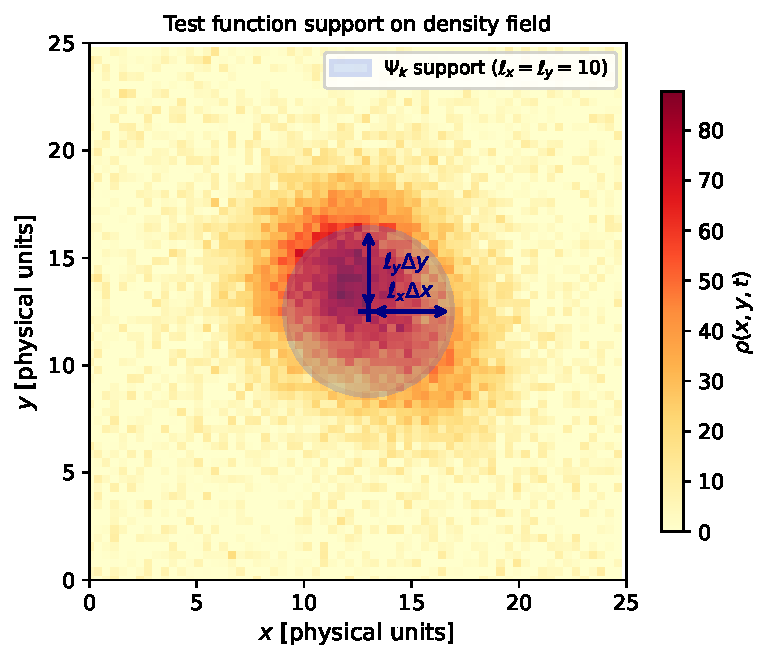
\includegraphics[width=0.72\textwidth]{../Thesis_Figures/fig8_test_footprint_2d}
\caption{Two-dimensional test function footprint overlaid on a representative
density field (gas regime, $t=10$\,s).  The shaded ellipse shows the spatial
support of a single test function $\Psi_k(x,y)=\psi_x(x)\psi_y(y)$ with
half-widths $(\ell_x\Delta x,\ell_y\Delta y)$ at the default scale
$\ell_x=\ell_y=10$.  The footprint covers several density wavelengths,
illustrating the spatial averaging implicit in the weak-form inner products.
Coarser $\ell$ suppresses high-frequency noise but smears sharp gradients;
finer $\ell$ resolves smaller features at the cost of noise amplification.
The support widths of the test functions should therefore be interpreted as
part of the discovered model scale: changing them changes which modes of the
data dominate the weak constraints, and therefore changes the effective PDE
that is recoverable.}
\label{fig:test_footprint_2d}
\end{figure}

\subsection{Integration by parts}
\label{subsec:ibp}

Consider the PDE $u_t = F(u)$ on the periodic spatial domain
$\Omega=[0,L_x)\times[0,L_y)$ over the time interval
$[0,T]$.  For a test function $\psi_k$ centred at a query point
$(x_k,y_k,t_k)$, let $Q_k := \operatorname{supp}\psi_k
\subset \Omega\times[0,T]$ denote its spacetime support, with
half-widths $(\ell_t\Delta t,\ell_x\Delta x,\ell_y\Delta y)$.
Multiplying both sides
by $\psi_k$ and integrating over~$Q_k$ gives
\[
  \int_{Q_k} \psi_k(x,y,t)\,u_t(x,y,t)\;dx\,dy\,dt
  = \int_{Q_k} \psi_k(x,y,t)\,F(u)(x,y,t)\;dx\,dy\,dt.
\]
Equivalently, since $\psi_k$ vanishes outside~$Q_k$, one may view these as
integrals over the full spacetime domain $\Omega\times[0,T]$.  Integrating
the left side by parts in time, the temporal boundary term vanishes because
$\psi_k$ is compactly supported in time (i.e.\ $\psi_k$ vanishes at the
temporal endpoints of~$Q_k$):
\begin{equation}
  -\int_{Q_k} \frac{\partial\psi_k}{\partial t}(x,y,t)\,u(x,y,t)\;dx\,dy\,dt
  = \int_{Q_k} \psi_k(x,y,t)\,F(u)(x,y,t)\;dx\,dy\,dt.
  \label{eq:ibp_temporal}
\end{equation}
Likewise, for differential operators appearing in~$F(u)$, spatial
integration by parts transfers derivatives from the data~$u$ onto the test
function~$\psi_k$.  Under periodic boundary conditions on~$\Omega$, the
spatial boundary contributions vanish (by a distinct mechanism: periodicity,
not compact support).  For example, if $F(u)$ contains a
term $w_m\,\Delta u$, then
\[
  w_m\int_{Q_k}\psi_k\,\Delta u\;dx\,dy\,dt
  = -\,w_m\int_{Q_k}\nabla\psi_k\cdot\nabla u\;dx\,dy\,dt
  = w_m\int_{Q_k}(\Delta\psi_k)\,u\;dx\,dy\,dt,
\]
where the intermediate equality follows from two spatial integrations by
parts with periodic boundary terms vanishing.  Thus the data~$u$ always appears
\emph{undifferentiated}.  The one-dimensional bump formula
\eqref{eq:test_1d} is analytic, but the sampled derivative arrays used in
the weak system are evaluated numerically on the discrete support lattice
via one-dimensional finite-difference stencils and then assembled by
separable outer products.
Although the bump formula is analytic and admits closed-form derivatives,
numerical evaluation on the sampled lattice avoids special-casing outside
the general-purpose convolution pipeline and introduces errors that are
negligible relative to the test-function support scale.

\begin{figure}[htbp]
\centering
\begin{tikzpicture}[
    box/.style={draw, rounded corners, minimum width=3.2cm, minimum height=2.4cm, align=center},
    arrow/.style={->, >=stealth, thick},
  ]
  % Left box: noisy data
  \node[box] (data) at (0,0) {%
    \textbf{Noisy data $u$}\\[4pt]
    \begin{tikzpicture}[scale=0.5]
      \draw[blue, thick] plot[smooth, domain=0:3.5, samples=60]
        (\x, {sin(2*\x r) + 0.3*rand});
    \end{tikzpicture}
  };
  % Right box: smooth test derivative
  \node[box] (test) at (7.5,0) {%
    \textbf{Smooth $\partial\psi/\partial t$}\\[4pt]
    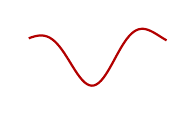
\begin{tikzpicture}[scale=0.5]
      \draw[red!70!black, thick] plot[smooth, domain=0:3.5, samples=60]
        (\x, {cos(2*\x r)*exp(-0.5*(\x-1.75)*(\x-1.75))});
    \end{tikzpicture}
  };
  % Arrow
  \draw[arrow] (data) -- node[above, font=\small] {IBP} node[below, font=\footnotesize, text width=3cm, align=center] {transfers derivatives\\onto known $\psi$} (test);
  % Bottom annotation
  \node[below=0.6cm of data.south east, anchor=north, text width=10cm, align=center, font=\small\itshape] at (3.75,-1.8)
    {Result: all derivatives act on the analytic, smooth $\psi$, never on the noisy~$u$.};
\end{tikzpicture}
\caption{Schematic of the weak-form integration-by-parts mechanism.  The
noisy field data~$u$ (left) enters the inner product undifferentiated,
while all spatial and temporal derivatives are transferred to the
compactly supported, analytic test function~$\psi$ (right).  This
derivative transfer is the key regularisation that enables stable
regression from noisy data without explicit filtering or finite-difference
stencils on~$u$.
}
\label{fig:ibp_geometry}
\end{figure}

\subsection{Separability and FFT convolution}
\label{subsec:fft_conv}

Because $\psi_k$ is separable~\eqref{eq:test_separable}, each
three-dimensional integral reduces to a product of one-dimensional
convolutions, computed efficiently via the Fast Fourier Transform.
The spatial dimensions are periodic and use circular convolution;
the temporal dimension is zero-padded to avoid wrap-around artefacts.

% ======================================================================
\section{Candidate library construction}
\label{sec:library}

The library specifies which physical mechanisms the regression is allowed
to select.  Each candidate term is a pair $(\mathcal{L}_m, f_m)$
consisting of a differential operator~$\mathcal{L}_m$ and a pointwise
nonlinear feature~$f_m$.  Conceptually, the terms fall into five blocks:
\emph{transport and continuity backbone}
(e.g.\ $\nabla\!\cdot\!\mathbf{p}$),
\emph{diffusive regularisation}
(e.g.\ $\Delta\rho$, $\Delta p_x$),
\emph{alignment-related polarisation terms}
(e.g.\ linear drag $p_x$, cubic saturation $|\mathbf{p}|^2 p_x$),
\emph{nonlocal interaction terms from Morse forcing}
(e.g.\ $\rho\,\partial_x\Phi$, $\nabla\!\cdot\!(\rho\nabla\Phi)$),
and \emph{closure surrogates}
(e.g.\ $\partial_x(\rho^2)$ as a congestion proxy).

\subsection{Scalar library}
\label{subsec:scalar_library}

For a single field~$u$ the default library is the Cartesian product of
polynomial features and spatial operators:
\begin{equation}
  \bigl\{f_j\bigr\} = \{1,\;u,\;u^2,\;u^3\},
  \qquad
  \bigl\{\mathcal{L}_j\bigr\}
  = \{I,\;\partial_x,\;\partial_y,\;\Delta\},
  \label{eq:scalar_library}
\end{equation}
yielding up to 16 candidate terms (e.g.\ $\Delta u^2$, $\partial_x u$).
The maximum polynomial power is controlled by $p_{\max}$ (default~$3$)
and the operator set is configurable.  Optional extensions
include
nonlinear diffusion terms $\Delta(u^p)$ for specified powers~$p$,
gradient nonlinearities $|\nabla u|^2 = u_x^2+u_y^2$,
and conservative forms $\partial_x(u^p),\;\partial_y(u^p)$.
The library is assembled programmatically via a fluent builder pattern.

\subsection{Multi-field library for coupled Vicsek--Morse dynamics}
\label{subsec:multifield_library}

When multiple coarse-grained fields are available
(see \S\ref{sec:multifield_cg} for field definitions), the pipeline
discovers a coupled PDE system.  For the Vicsek--Morse model~\cite{vicsek1995vicsek,dorsogna2006morse} with
density~$\rho$, polarisation flux $(p_x,p_y)$, and Morse
potential~$\Phi=W*\rho$, three separate regressions share a common
test-function bundle but have independent candidate libraries.

Table~\ref{tab:multifield_terms} lists the default term set for each
equation.  The Morse potential is precomputed via FFT convolution of the
density with the radial kernel
$W(r) = -C_r e^{-r/\ell_r} + C_a e^{-r/\ell_a}$
(see~\eqref{eq:morse_fr}).

\begin{table}[ht]
\centering
\caption{Default multi-field library terms for the Vicsek--Morse system
(see accompanying repository for implementation details).}
\label{tab:multifield_terms}
\renewcommand{\arraystretch}{0.95}
\setlength{\tabcolsep}{8pt}
\begin{tabular}{lll}
\toprule
\textbf{Equation} & \textbf{Term name} & \textbf{Mathematical form} \\
\midrule
\multirow{6}{*}{$\rho_t = \cdots$}
  & \cv{div\_p}            & $\nabla\!\cdot\mathbf{p}$ \\
  & \cv{lap\_rho}          & $\Delta\rho$ \\
  & \cv{lap\_rho2}         & $\Delta(\rho^2)$ \\
  & \cv{lap\_rho3}         & $\Delta(\rho^3)$ \\
  & \cv{div\_rho\_gradPhi} & $\nabla\!\cdot(\rho\,\nabla\Phi)$ \\
  & \cv{lap\_p\_sq}        & $\Delta(|\mathbf{p}|^2)$ \\
\midrule
\multirow{8}{*}{$(p_x)_t = \cdots$}
  & \cv{px}                & $p_x$ \\
  & \cv{p\_sq\_px}         & $|\mathbf{p}|^2\,p_x$ \\
  & \cv{dx\_rho}           & $\partial_x\rho$ \\
  & \cv{dx\_rho2}          & $\partial_x(\rho^2)$ \\
  & \cv{lap\_px}           & $\Delta p_x$ \\
  & \cv{bilap\_px}         & $\Delta^2 p_x$ \\
  & \cv{rho\_dx\_Phi}      & $\rho\,\partial_x\Phi$ \\
  & \cv{div\_px\_p}  & $\nabla\!\cdot\!(p_x\,\mathbf{p})$ \\
\midrule
$(p_y)_t = \cdots$ & \multicolumn{2}{l}{\emph{(analogous to $p_x$ with $x\leftrightarrow y$)}} \\
\bottomrule
\end{tabular}
\end{table}

The $\rho$-equation terms encode diffusion, nonlinear diffusion, and
Morse-mediated drift; the momentum equations add linear drag ($p_x$),
cubic self-interaction ($|\mathbf{p}|^2 p_x$), pressure-like gradients
($\partial_x\rho$), viscosity ($\Delta p_x$), hyper-viscosity
($\Delta^2 p_x$), Morse forcing ($\rho\,\partial_x\Phi$), and
self-advection ($\nabla\!\cdot\!(p_x\,\mathbf{p})$).

Table~\ref{tab:rosetta_stone} maps each library term to the
microscopic particle mechanism it encodes, providing a reference
for interpreting the coefficient results in Chapter~\ref{ch:wsindy_results}.

\begin{table}[ht]
\centering
\caption{``Rosetta Stone'' mapping from microscopic particle mechanisms to
continuum-level library terms.  This table bridges the gap between
the agent-based model (Chapter~\ref{ch:experimentation}) and the discovered PDEs
(Chapter~\ref{ch:wsindy_results}), making explicit the physical interpretation of each library
column.  Empirical recovery results (which regimes activate which terms) are
reported in Chapter~\ref{ch:wsindy_results}
(Table~\ref{tab:mechanism_confidence}).}
\label{tab:rosetta_stone}
\renewcommand{\arraystretch}{0.95}
\begin{tabular}{p{3.8cm}p{4.0cm}p{3.0cm}}
\toprule
\textbf{Microscopic mechanism} & \textbf{Continuum form} & \textbf{Library term} \\
\midrule
Vicsek alignment      & $-\alpha\,p_x$          & \texttt{px}             \\
Compressible transport & $\nabla\cdot\mathbf{p}$ & \texttt{div\_p}         \\
Viscous regularisation & $\Delta p_x$            & \texttt{lap\_px}        \\
Momentum self-advection & $\nabla\cdot(p_x\,\mathbf{p})$ & \texttt{div\_px\_p} \\
Morse attraction      & $\rho\,\nabla\Phi$       & \texttt{rho\_dx\_Phi}   \\
Morse repulsion       & $-\rho\,\nabla\Phi$ (sign flip) & \texttt{rho\_dx\_Phi} \\
Density-dependent pressure & $\partial_x(\rho^2)$ & \texttt{dx\_rho2}      \\
Density diffusion     & $\Delta\rho$             & \texttt{lap\_rho}       \\
Aggregation correction & $\nabla\cdot(\rho\,\nabla\Phi)$ & \texttt{div\_rho\_gradPhi} \\
\bottomrule
\end{tabular}
\end{table}

% ======================================================================
\section{Weak linear system assembly}
\label{sec:weak_system}

Given a density snapshot tensor $U\in\mathbb{R}^{T\times n_x\times n_y}$
and a collection of $K$~test functions $\{\psi_k\}_{k=1}^K$, the weak
formulation~\eqref{eq:ibp_temporal} produces the overdetermined linear
system
\begin{equation}
  \mathbf{b} = \mathbf{G}\,\mathbf{w},
  \qquad
  \mathbf{b}\in\mathbb{R}^K,\;
  \mathbf{G}\in\mathbb{R}^{K\times M},\;
  \mathbf{w}\in\mathbb{R}^M,
  \label{eq:weak_system}
\end{equation}
with components defined as follows.

\noindent\textbf{Left-hand side (temporal derivative).}
Each entry of~$\mathbf{b}$ encodes the time derivative transferred
onto the test function:
\begin{equation}
  b_k = -\sum_{x,y,t}
    \frac{\partial\psi_k}{\partial t}(x,y,t)\;
    U(x,y,t)\;
    \Delta x\,\Delta y\,\Delta t.
  \label{eq:b_vector}
\end{equation}
The one-dimensional bump functions are defined analytically by
\eqref{eq:test_1d}, but the discrete derivative arrays entering
$\partial_t\psi_k$ are evaluated numerically on the support lattice via
one-dimensional finite-difference stencils and then assembled by
separable outer products.

\noindent\textbf{Right-hand side (library evaluations).}
For each library term $(\mathcal{L}_m,f_m)$, the $(k,m)$-entry of the
design matrix~$\mathbf{G}$ is
\begin{equation}
  G_{k,m}
  = \sum_{x,y,t}
    \bigl(\mathcal{L}_m[\psi_k]\bigr)(x,y,t)\;
    f_m\!\bigl(U(x,y,t)\bigr)\;
    \Delta x\,\Delta y\,\Delta t,
  \label{eq:G_matrix}
\end{equation}
where $\mathcal{L}_m[\psi_k]$ denotes the \emph{adjoint} of operator
$\mathcal{L}_m$ applied to the test function (e.g.\ $\Delta\psi_k$ for
the Laplacian, $-\partial_x\psi_k$ for $\partial_x$ under periodic BC).

\noindent\textbf{Query-point selection.}
The $K$ test functions are centred at a uniform sub-grid with strides
$(s_t,s_x,s_y)$ (default $(2,2,2)$).  A temporal margin
of $\ell_t$~time steps is excluded at the beginning and end of the
time series to keep each test function's support within the data domain.
The resulting system is tall and thin ($K\gg M$), well-suited for
least-squares regression.  Query points are sampled uniformly over the admissible spacetime region; no adaptive weighting toward high-gradient regions was used.

\noindent\textbf{Implementation.}
All convolutions in \eqref{eq:b_vector}--\eqref{eq:G_matrix} are
evaluated via 3-D FFT convolution (see \S\ref{subsec:fft_conv})
and then sampled at the query locations.

\noindent\textbf{Separability of the test functions.}
Because $\Psi_k(t,x,y)=\psi_t^{(k)}(t)\,\psi_x^{(k)}(x)\,\psi_y^{(k)}(y)$,
each three-dimensional convolution factors into three
one-dimensional convolutions computed via FFT in
$\mathcal{O}(N\log N)$ time per axis.  The factored form reduces peak memory
since only one axis is buffered at a time, and the same separability applies
to every adjoint differential operator in the library.

\noindent\textbf{Multiple trajectories.}
In practice, WSINDy is fit from many training simulations sharing the same
parameter regime but differing in initial condition.  These trajectories are
\emph{not} concatenated end-to-start into one artificial long time series.
Instead, for each trajectory $c=1,\dots,C$ we assemble a separate weak system
$\mathbf{b}^{(c)} = \mathbf{G}^{(c)}\mathbf{w}$,
and then stack the resulting rows into one global regression problem,
\begin{equation}
  \begin{bmatrix}
    \mathbf{b}^{(1)}\\
    \mathbf{b}^{(2)}\\
    \vdots\\
    \mathbf{b}^{(C)}
  \end{bmatrix}
  =
  \begin{bmatrix}
    \mathbf{G}^{(1)}\\
    \mathbf{G}^{(2)}\\
    \vdots\\
    \mathbf{G}^{(C)}
  \end{bmatrix}
  \mathbf{w}.
  \label{eq:stacked_weak_system}
\end{equation}
This yields one common sparse coefficient vector for the scalar case.  In the
multi-field Vicsek--Morse setting, the same block-stacking idea is applied
separately to the $\rho$, $p_x$, and $p_y$ equations, producing three coupled
field-level regressions rather than a POD latent time-stepper.

% ======================================================================
\section{Sparse regression and model selection}
\label{sec:regression}

Sparsity-promoting regression originates with the Lasso; in the PDE-discovery context, the same principle underpins both SINDy's sequential thresholded least squares~\cite{brunton2016sindy} and the SR3 relaxation~\cite{zheng2019sr3}.

\subsection{Column preconditioning}
\label{subsec:precondition}

Library terms have physical magnitudes spanning several orders.
Without column preconditioning, dominant-balance thresholding would
preferentially retain large-magnitude terms regardless of explanatory
power, so we normalise each column to unit $\ell^2$ norm before
regression.

Before thresholding, each column of $\mathbf{G}$ is normalised to unit
$\ell^2$ norm:
\begin{equation}
  \tilde{G}_{:,j} = G_{:,j}\,/\,s_j,
  \qquad
  s_j = \lVert G_{:,j}\rVert_2,
  \label{eq:precondition}
\end{equation}
so that the thresholding criterion treats all candidate terms on equal
footing regardless of their physical scale.  After regression on the
normalised system $\tilde{\mathbf{G}}\tilde{\mathbf{w}}\approx\mathbf{b}$,
the physical coefficients are recovered by $w_j = \tilde{w}_j/s_j$.

\subsection{MSTLS: dominant-balance thresholding}
\label{subsec:mstls}

We use the \emph{Multi-Step Thresholded Least Squares} (MSTLS) algorithm
with the dominant-balance criterion~\cite{callaham2021dominant}.
The sequential thresholding loop originates in the WSINDy framework of
Messenger and Bortz~\cite{messenger2021wsindy}; the dominant-balance
extension that replaces a fixed threshold with a relative-contribution
band is due to Minor et al.~\cite{minor2025mstls}.
Starting from all terms active, the algorithm iterates:
\begin{enumerate}[nosep]
\item Solve least squares on the active columns:
      $\tilde{\mathbf{w}}_{\mathcal{A}}
       = \arg\min_{\mathbf{w}}
         \lVert\tilde{\mathbf{G}}_{:,\mathcal{A}}\,\mathbf{w}
               -\mathbf{b}\rVert_2$.
\item Keep term~$j$ if its relative contribution lies in the band
      \begin{equation}
        \hat\lambda
        \;\le\;
        \Pi_j
        \;\le\;
        \frac{1}{\hat\lambda},
        \qquad
        \Pi_j := \frac{|\tilde{w}_j|\;\lVert\tilde{G}_{:,j}\rVert_2}
                      {\lVert\mathbf{b}\rVert_2},
        \label{eq:dominant_balance}
      \end{equation}
\item Repeat until the active set~$\mathcal{A}$ converges
      (or a maximum of 25 iterations).
\end{enumerate}
The procedure is run for each threshold in a logarithmic grid
$\hat\lambda\in[10^{-4},10^1]$ (40 values), and the threshold
producing the lowest normalised loss is selected (ties broken
by sparsity).  Full pseudocode is given in
Algorithm~\ref{alg:mstls} (Appendix~\ref{app:mstls}), which details
the threshold sweep, dominant-balance scoring, and iterative
re-solve loop.

\subsection{Automated model selection across test-function scales}
\label{subsec:model_selection}

The accuracy of the weak formulation depends critically on the test-function
half-widths $\boldsymbol\ell=(\ell_t,\ell_x,\ell_y)$: too narrow yields
noisy convolutions; too wide smooths out spatial structure.  Rather than
selecting $\boldsymbol\ell$ by hand, we sweep a log-spaced grid of
configurations (typically 5--20 trials) and score each with a composite
objective:
\begin{equation}
  S(\boldsymbol\ell)
  = L_{\mathrm{norm}}(\boldsymbol\ell)
  + \alpha\,\frac{n_{\mathrm{active}}(\boldsymbol\ell)}{M}
  + \beta\,\max\!\Bigl(0,\;
      \log_{10}\kappa(\boldsymbol\ell)
      - \log_{10}\kappa_0\Bigr),
  \label{eq:composite_score}
\end{equation}
where $L_{\mathrm{norm}}$ is the MSTLS normalised residual
($L_{\mathrm{norm}} = \lVert\mathbf{b} - \tilde{\mathbf{G}}\tilde{\mathbf{w}}^*\rVert_2
 / \lVert\tilde{\mathbf{G}}\mathbf{w}_{\mathrm{LS}}\rVert_2$,
i.e.\ the residual relative to the unconstrained least-squares fit),
$n_{\mathrm{active}}$ the number of surviving terms, $M$ the total library
size, and $\kappa$ the condition number of the active sub-matrix
($\kappa(\mathbf{A}) = \sigma_{\max}(\mathbf{A})/\sigma_{\min}(\mathbf{A})$).  The
default weights are $\alpha=0.1$ (complexity penalty), $\beta=0.01$
(conditioning penalty), and $\kappa_0=10^8$ (threshold above which
conditioning is penalised).

The choice $\alpha=0.1$ was selected empirically and verified
robust to perturbations in $[0.05,\,0.2]$
(Section~\ref{subsec:tf_sensitivity}, Chapter~\ref{ch:wsindy_results}).
The conditioning penalty~$\beta$ acts as a soft safeguard: it has no
effect until $\kappa$ exceeds $\kappa_0$, after which it linearly
penalises further ill-conditioning.  In practice, $\beta$ triggers only
when two or more library terms are near-collinear (e.g.\ $\rho\nabla^2\rho$
and $|\nabla\rho|^2$ in low-resolution regimes).  Robustness of the
selected models to moderate perturbations of both weights
is verified empirically in Section~\ref{subsec:tf_sensitivity}
(Chapter~\ref{ch:wsindy_results}).

The configuration minimising~\eqref{eq:composite_score} is returned as the
best model.  A Pareto frontier in the two-dimensional space
$(L_{\mathrm{norm}},\;n_{\mathrm{active}})$ is also computed for
user inspection.

The model selection sweep, composite scoring, and Pareto-frontier
extraction are provided in the accompanying repository.

% ======================================================================
\section{Uncertainty quantification}
\label{sec:uq}

\subsection{Bootstrap resampling}
\label{subsec:bootstrap}

To quantify coefficient uncertainty, we resample the $K$~rows of the weak
system $(\mathbf{b},\mathbf{G})$ uniformly at random with replacement,
refit MSTLS on each bootstrap replicate, and collect the resulting
coefficient vectors~\cite{messenger2021wsindy}:

\begin{enumerate}[nosep]
\item For $b=1,\dots,B$ (default $B=100$):
  \begin{enumerate}[nosep]
  \item Draw $K'=\lceil K\cdot f_{\mathrm{sub}}\rceil$ rows with
        replacement (default $f_{\mathrm{sub}}=1$).
  \item Refit MSTLS $\to$ $\mathbf{w}^{(b)}$, active set $\mathcal{A}^{(b)}$.
  \end{enumerate}
\item Aggregate:
  \begin{itemize}[nosep]
  \item Mean $\bar{w}_j = \frac{1}{B}\sum_b w_j^{(b)}$,\;
        Std $\sigma_j = \sqrt{\frac{1}{B}\sum_b(w_j^{(b)}-\bar{w}_j)^2}$.
  \item Inclusion probability
        $P_j = \frac{1}{B}\sum_b\mathbf{1}_{j\in\mathcal{A}^{(b)}}$.
  \item Percentile-based confidence intervals (default 95\%).
  \end{itemize}
\end{enumerate}

\subsection{Stability selection}
\label{subsec:stability}

Stability selection~\cite{meinshausen2010stability} identifies which
discovered terms are robust to changes in the test-function scale and/or
the data subsample.  For each configuration~$c$ in a set of $n_c$~trials
(varying $\boldsymbol\ell$ and, optionally, bootstrap subsamples):
\begin{enumerate}[nosep]
\item Build the weak system for configuration~$c$.
\item Fit MSTLS and record the active set $\mathcal{A}^{(c)}$.
\end{enumerate}
The selection frequency of term~$j$ is
\begin{equation}
  f_j = \frac{1}{n_c}\sum_{c=1}^{n_c}\mathbf{1}_{j\in\mathcal{A}^{(c)}}.
  \label{eq:stability_freq}
\end{equation}
Terms are classified as
\emph{robust} ($f_j\ge 0.6$),
\emph{fragile} ($0<f_j<0.6$), or
\emph{never selected} ($f_j=0$).
The threshold 0.6 follows the recommendation of
Meinshausen \& B\"uhlmann~\cite{meinshausen2010stability}; it is a heuristic
criterion for robustness, not a theorem that partitions truth from falsehood.

\subsection{Weak-form coefficient of determination}
\label{subsec:r2wf}

We quantify instantaneous identification fit by the weak-form coefficient of determination
\begin{equation}
  R^2_{\mathrm{wf}}
  \;:=\;
  1 \;-\;
  \frac{\lVert\mathbf{b} - \mathbf{G}\mathbf{w}^*\rVert_2^2}
       {\lVert\mathbf{b}\rVert_2^2},
  \label{eq:r2wf}
\end{equation}
where $\mathbf{b}$ is the weak-form right-hand side and
$\mathbf{G}\mathbf{w}^*$ the fitted weak-form prediction.
The denominator is the uncentred signal energy, not the variance about
the mean; this convention is appropriate because the weak system has
already been zero-centred by the test-function projection.
Unlike forecast~$R^2$, which measures predictive accuracy over a rollout
horizon, $R^2_{\mathrm{wf}}$ is an identification metric in weak
residual space: it reports how well the selected library terms explain
the instantaneous PDE residual on the training data.

% ======================================================================
\section{PDE forecasting as a closure stress test}
\label{sec:forecast}

Forward integration exposes closure limitations: divergence signals an
unclosed library rather than failed identification
(Section~\ref{sec:closure_problem}).
Once a sparse PDE has been identified, we integrate it forward in time
from a given initial condition to produce a density forecast.

\subsection{Strong-form RHS evaluation}
\label{subsec:rhs}

The right-hand side of the discovered PDE is evaluated pointwise in
physical space:
\begin{equation}
  u_t(x,y)
  = \sum_{m\in\mathcal{A}} w_m\;\mathcal{L}_m\!\bigl[f_m(u)\bigr](x,y),
  \label{eq:rhs_eval}
\end{equation}
where spatial derivatives are computed spectrally via FFT on the periodic
domain:
$\widehat{\partial_x u}(k_x,k_y) = i\,k_x\,\hat{u}(k_x,k_y)$
and
$\widehat{\Delta u}(k_x,k_y) = -(k_x^2+k_y^2)\,\hat{u}(k_x,k_y)$.

\subsection{Linear--nonlinear splitting}
\label{subsec:splitting}

To enable exponential time-stepping, the discovered RHS is decomposed into
\begin{equation}
  u_t = L\,u + N(u),
  \label{eq:lin_nonlin_split}
\end{equation}
where $L$ collects all terms that are \emph{linear} in~$u$ (feature $=u$,
any operator, e.g.\ $\alpha\Delta u$, $\beta\partial_x u$) and $N(u)$
contains the nonlinear remainder (e.g.\ $\Delta u^2$, $|\nabla u|^2$).
In Fourier space, $L$ has a diagonal multiplier
\begin{equation}
  \hat{L}(k_x,k_y)
  = \sum_{m\in\mathcal{A}_{\mathrm{lin}}} w_m\,\sigma_m(k_x,k_y),
  \label{eq:L_hat}
\end{equation}
where $\sigma_m$ is the Fourier symbol of operator~$\mathcal{L}_m$
(e.g.\ $\sigma_{\Delta}=-(k_x^2+k_y^2)$, $\sigma_{\partial_x}=ik_x$).
This splitting is performed automatically during forecast initialisation.

\subsection{ETDRK4 integration}
\label{subsec:etdrk4}

When a linear component exists, we use the fourth-order exponential
time-differencing Runge--Kutta scheme (ETDRK4) of Cox \&
Matthews~\cite{cox2002etdrk}, stabilised with the contour-integral trick
of Kassam \& Trefethen~\cite{kassam2005etdrk4}.  The scheme treats the
linear part \emph{exactly} in Fourier space via matrix exponentials, so
that the time-step is not constrained by diffusive CFL limits.  The
nonlinear terms are integrated with fourth-order accuracy through four
sub-stage evaluations.  Full coefficient formulas and the per-step
algorithm are given in Appendix~\ref{app:etdrk4}, which tabulates the
four sub-stage weights and the contour-integral evaluation of the matrix
exponential coefficients.

When no linear terms are present, a classical fourth-order Runge--Kutta
(RK4) integrator is used as a fallback.

\noindent\textbf{High-level interface.}
The forecast routine
selects the integrator automatically: ETDRK4 when
linear terms exist, RK4 otherwise.  An optional density floor
enforces $u\ge 0$ after each time step.

% ======================================================================
\section{Physical inductive biases}
\label{sec:pipeline_fixes}
% ======================================================================

Six physical inductive biases were incorporated after a
post-implementation audit.  Each targets a specific numerical artefact,
non-physical operator, or degenerate optimisation mode identified during
trial runs.  All six are active regardless of YAML configuration.
We group them by how they intervene in the identification pipeline.

\paragraph{Library-structure biases.}
\emph{Biharmonic operator removal.}
The biharmonic operator~$\nabla^4$ was removed from the candidate library.
In trial runs it absorbed energy from the physically motivated viscous
term~$\Delta p_x$, producing a higher-order regularisation with no
counterpart in the expected mean-field structure.  Its removal restricts
the library's expressivity but prevents a known degeneracy; the remaining
library still spans all mechanisms listed in Table~\ref{tab:multifield_terms}.
\emph{Regime-aware library construction.}
A regime-specific flag controls whether Morse potential terms enter
the candidate library; for pure-Vicsek regimes the Morse columns are
automatically excluded, preventing the regression from fitting interaction
artefacts where no interaction force exists.  This is the only bias that
uses regime metadata.

\paragraph{Post-fit filters.}
\emph{Sign constraints on post-fit coefficients.}
After each MSTLS solve, coefficients whose physical sign is known
\emph{a priori} (viscous terms must be non-positive, ensuring
dissipation rather than anti-diffusion) are checked; sign-violating
survivors are zeroed and the fit is re-solved.
\emph{Coefficient magnitude cap.}
Retained coefficients exceeding $|c|>5.0$ are removed, guarding against
inflation from near-singular library matrices or ill-conditioned
regression subproblems.  The threshold was set conservatively above the
largest physically plausible coefficient observed across regimes.
Because both filters act \emph{after} the sparse selection step, they
cannot introduce terms that the data did not select; they can only
remove terms that violate known physics.

\paragraph{Preprocessing biases.}
\emph{Centred flux estimation.}
The KDE flux estimator subtracts the domain-mean flux from each snapshot
before weak-form convolution.  Without this correction, a nonzero mean
flux arising from net flock translation aliases into the linear drag
coefficient~$p_x$, producing a spurious offset that distorts the momentum
equation's relaxation structure.  The correction removes a numerical
artefact without constraining which terms the regression selects.
\emph{Temporal test-function width floor.}
The temporal support is floored at $\ell_t \geq 7$ grid points.  Without
this floor, the composite-score width optimiser can collapse the temporal
integral to near-pointwise evaluation, reintroducing the derivative-noise
sensitivity that the weak form is designed to avoid.  The floor value was
chosen empirically as the smallest support that yields stable coefficient
estimates across regimes.

\paragraph{Summary and scope of intervention.}
The first two biases (biharmonic removal, regime-aware library) genuinely
constrain what the regression can discover by excluding specific library
columns.  The post-fit filters (sign, magnitude) constrain the regression
output but cannot introduce new terms.  The preprocessing biases (flux
centring, temporal floor) condition the input data without altering the
library.  Each targets a previously identified numerical artefact; within
the admissible library that remains after these interventions, the
selection of active terms is fully data-driven via MSTLS sparsification.

\paragraph{Chapter summary.}
The pipeline described above fixes the complete identification protocol:
separable weak-form test functions transfer derivatives away from noisy
data, a physically motivated candidate library constrains what can be
discovered, MSTLS with dominant-balance thresholding enforces sparsity,
and composite-score model selection ensures that the result is robust to
the test-function scale.  Bootstrap UQ and stability selection provide
the uncertainty characterisation needed to distinguish reliably recovered
backbone terms from fragile artefacts.  In
Chapter~\ref{ch:wsindy_results}, a discovered PDE will be considered
\emph{successfully identified} when it meets the four criteria stated at
the opening of this chapter; autonomous rollout is reported as a closure
diagnostic, not as the primary measure of identification quality.
